\documentclass{article}
\usepackage[utf8]{inputenc}

\usepackage{biblatex}
\bibliography{robustness.bib}

\usepackage{bm}
\usepackage{amsmath}

\usepackage{graphicx}

\title{Multivariate robustness in gene networks}
\author{Arnaud LE ROUZIC}
\date{}

\begin{document}

\maketitle

\section{Introduction}

Predicting how genotypes map to phenotypes is of outstanding interest in most life sciences. Decades of progress in genetics and in cell, molecular, developmental, and systems biology, have considerably improved our understanding of the mechanisms involved in the genotype-to-phenotype relationship. However, if we can explain why the genoype-phenotype link is complex, whether or not (and how) accounting for this complexity in evolutionary thinking is still debated. 

Paradoxically, the most efficient models in evolutionary and quantitative genetics (both in terms of predictive and explanatory power) are based on a statistical abstraction of genetic effects in which allele

\section{Model and Methods}

\subsection{Gene regulatory network}

The network model is derived from \cite{Wag94,Wagner96} and belongs to the family of GRN sometimes refered to as "Wagner model" (see \cite{FierstPhuillips2016} for the historical record). The main difference with the original Wagner model is that the network output (gene expressions) is quantitative and not qualitative, in the same way as in \cite{SB02}. 

More specifically, the structure of a $n$-gene network is encoded as a $n\times n$ matrix $\bm W$, while the state of the network is stored into a vector of size $n$, $\bm S$. In this setting, $W_{ij}$ represents the influence of gene $j$ on the expression of gene $i$, $W_{ij} < 0$ represents a negative interaction (inhibition), $W_{ij} > 0$ a positive interaction (activation), and $W_{ij} = 0$ denotes the absence of regulatory interaction. $S_i$ is the expression of gene $i$, ranging between 0 (no expression) and 1 (maximum expression). 

The properties of these gene networks are explored in a discrete dynamic system:
\begin{equation}
 \bm S_{t+1} = F(\bm W \bm S_t),
\end{equation}
\noindent where the function $F$ is a vectorized version of a sigmoid scaling function: $F(x_1, x_2, \dots, x_n) = [f(x_1), f(x_2), \dots, f(x_n)]$ with
\begin{equation} \label{eq:fx}
f(x) = \frac{1}{1+ \lambda_a e ^{- \mu_a x}}, 
\end{equation}
\noindent with $\lambda_a = (1-a)/a$ and $\mu_a = 1/a(1-a)$. The function $f$ is scaled such that $f(0) = a$ and $df/dx|_{x=0}=1$; the parameter $a$ thus stands for the constitutive gene expression (the expression of a gene that is not regulated), and this function defines the scale of the matrix $\bm W$, as a small effect $W_{ij} = \delta$ on an otherwise non-regulated gene leads to the same change in gene expression $S_i = a+\delta$. Setting $a=0.5$ leads to $f(x) = 1/(1+e^{-\mu x})$ with $\mu = 4$, which can be directly compared with e.g.\ \cite{PBF12}. 

Gene networks start with an initial expression $S_0$ and were run for $T$ timesteps. By default, $S_0 = (a, a, ..., a)$, since this step immediately follows a virtual initial state with no expression. The expression phenotype corresponding to a gene network was determined by averaging gene expressions during the last $\tau$ timesteps for each gene $i$: $\bar S_i = \sum_{t=T-\tau}^T S_{it}$. 

\subsection{Robustness indicators}

Five robustness indicators were calculated, corresponding to five different aspects of genetic or environmental robustness in a gene network: the network stability $U$, the network homeostasis $H$, the environmental canalization $E$, the genetic canalization $C$, and the somatic canalization $K$. 

Network stability $U$ refers to the capacity for a specific network to lead to stable gene expression. Indeed, dynamic systems based on the Wagner model often tend to generate limit cycles and never converge to a stable equilibrium. For consistency with other indicators, this unstability was measured as the average deviation from the mean expression during the last $\tau$ timesteps: $U_i = \sum_{t=T-\tau}^T |S_{it}-\bar S_i| / \tau$. $U_i$ thus actually measures the unstability of gene $i$, as it reaches 0 for a stable gene and 0.5 for a totally unstable gene (cyclic switches between minimum and maximum expression levels). 

Homeostasis $H$ measures the capacity of a network to recover its equilibrium state after having being disturbed. In practice, gene expressions after $T$ timesteps were disturbed by adding a random Gaussian noise of standard deviation $\sigma_e$ to each gene of the network, and the homeostasis score $H$ was computed as the average difference between gene expression after disturbance $\bar S^\prime_{T+1}$ and the expression before disturbance $\bar{\bm S}$. The score was averaged over $R$ replicates and was measured independently for each gene i: $H_i = \sum_{r=1}^R | S^\prime_{i,T+1} - \bar S_i| / R$. 

Environmental canalization $E$ measures the capacity of a network to reach a consistent final state in spite of "developmental" disturbances. In practice, the initial state of the network $S_0$ was drawn into a (multivariate) uniform (0,1) distribution, and the average difference between the final state of disturbed ($\bar{\bm S}^\ast$) and undisturbed ($\bar{\bm S}$) networks reflect the robustness to the perturbation of the initial state. The procedure was replicated $R$ times, and $E_i = \sum_{r=1}^R |\bar S^\ast_{i}-\bar S_i|/R$. 

Genetic canalization $C$ measures the system robustness to genetic mutations (modifications of the $\bm W$ matrix). A random non-zero element of the $\bm W$ matrix was shifted by a random Gaussian number of standard deviation $\sigma_m$, and its consequences on the mean expression of all network genes $\bar{\bm S}^m$ was recorded. The procedure was replicated $R$ times, and $C_i = \sum_{r=1}^R |\bar S^m_i - \bar S_i| / R$. 

Finally, the Somatic canalization score $K$ merges the concepts of genetic canalization and homeostasis by measuring the impact of a mutation in the gene network $\bm W$ after having reached the final state. In practice, the $\bm W$ matrix was mutated in the same way as for genetic canalization, but its consequences on gene expression were calculated for only one timestep, starting from the final state of the network. The procedure was simulated $R$ times, and $K_i = \sum_{r=1}^R |S^m_{i,T+1} - \bar S_i|/R$. 

All these scores (including gene expressions) were calculated for every gene of the networks, but were also averaged over genes in order to get a series of summary network descriptors, noted $\bar{\bar S}, \bar U, \bar H, \bar E, \bar C,$ and $\bar K$. 

\subsection{Evolutionary simulations}

\subsection{Random networks}

Random networks were generated as $n\times n$ matrices filled with independent identically-distributed random numbers drawn into a Gaussian ($\mu_0, \sigma_0$) distribution. A density parameter $1/n \leq d \leq 1$ could be specified, corresponding to the frequency of non-zero slots in the $\bm W$ matrix. Zeros were placed randomly, with the constraint that all genes should be regulated by at least another one. 

In addition, 

\section{Results}

\subsection{Random networks}

Random interaction matrices are regularly used in the literature to study the general properties of gene networks (e.g.\ \cite{CTH11,PBF12}. As such, random networks are not expected to reflect the properties of biologically-realistic genetic architectures, as biological networks are far from random. However, such an approach helps developing a general intuition about the properties of the underlying model, especially about the amount of selection it takes to bring a network into its non-random state. 

Here, the point was to generate random networks displaying diversified behaviors in terms of robustness and canalization. Determining the random network parameters $\mu_0$ and $\sigma_0$ for such an analysis was, however, not trivial, as the parameter space optimizing robustness diversity did not overlap across robustness parameters. For instance, $\mu_0=0, \sigma_0=0.2$ offers a large diversity of genetic canalization scores, with both decanalized and canalized networks, but all networks are perfectly stable and environmentally canalized. The combination $\mu_0 = -0.2, \sigma_0 = 1.2$ was eventually retained as a reference parameter set for networks of size $n=6$, as it offers an acceptable compromise (Supplementary results~S1). 

Correlations were calculated between all five robustness components over 10,000 random networks (Figure~\ref{fig:cor}). All robustness components are positively correlated. However, correlations range from 0.9 (Homeostasis vs.\ Stability) to 0.2 (Homeostasis vs.\ Genetic Canalization), and in general tend to be rather weak. A Principal Component Analysis (Figure~\ref{pca}) confirms that robustness components are not tighly associated. The first PC (57\% of the total variance) corresponds to the general robustness/canalization of the network. The remaining variance is explained by orthogonal vectors separating Homeostasis/Stability vs.\ Genetic and Environmental Canalizations (PC2, 24\%), Genetic vs.\ Environmental Canalizations (11\%, PC3), Late mutations vs.\ all the rest (PC4, 7\%), and Stability vs.\ Homeostasis (PC5, 1\%). 

\subsection{2-gene networks}

The main interest of gene-network models is the complexity and the richness of the underlying genotype-phenotype. As a side effect, such models are particularly difficult to handle mathematically (see \cite{CTH11,LP12}). Excluding the one-gene self-regulating case (which already has non-trivial mathematical properties), the simplest network (2-by-2 matrix) has four genetic parameters, which precludes a tractable analysis. Here, I restricted the number of dimensions by considering the set of networks that lead to a predefined arbitrary equilibrium, $\bm S_\infty = (S_1, S_2)$. As $F(\bm W \bm S_\infty) = \bm S_\infty$, the $\bm W$ matrix can be reduced to two independent parameters, $W_{11}$ and $W_{21}$:
\begin{equation}
    \bm W = F \left [\begin{pmatrix} W_{11} & a \\ W_{21} & b \end{pmatrix}  \begin{pmatrix} S_1 \\ S_2 \end{pmatrix} \right] = \begin{pmatrix}S_1 \\ S_2 \end{pmatrix},
\end{equation}
\noindent with
\begin{equation}
    \begin{split}
        a = \frac{1}{S_2} [f^{-1}(S_1)-W_{11}S_1], \\
        b = \frac{1}{S_2} [f^{-1}(S_2) - W_{21} S_1],
    \end{split}
\end{equation}
\noindent $f^{-1}(x) = -\frac{1}{\mu_a} \log \left( \frac{1-x}{\lambda_a x} \right)$ being the inverse of $f(x)$ (equation~\ref{eq:fx}). The $\bm W$ matrix achieving the desired $\bm S_\infty$ equilibrium from a specific pair $W_{11}, W_{21}$ always exists (and is unique), but the stability of the equilibrium is not guaranteed. 

In the following, I considered the particular case of $\bm S_\infty$ = (0.3, 0.6) with two intermediate, distinct gene expressions. Equivalent results could be achieved with a different target. Figure~\ref{fig:imgpanels} illustrates how the robustness components vary in this constrained 2-gene network model (red stands for maximum robustness, i.e.\ minimum scores for $U$,$H$,$E$,$C$, and $K$). In the white regions, the equilibrium was not achieved in numerical simulations for distinct reasons. In the bottom-right region, the target $\S_\infty$ equilibrium was unstable, and the model converged to another equilibrium if the starting point was different from $\bm S_\infty$. In the top-left region, fluctuations around the equilibrium were so large that they hit the edges of the (0,1) gene expression interval, shifting the average gene expression towards 0.5. 

It immediately appears that the different robustness components may be somehow correlated, but do not overlap. The simulated behavior of networks A to E are illustrated in Figure~\ref{fig:simpanels}, and the corresponding $\bm W$ matrices are provided in Table~\ref{tab:W}. The network denoted as "B" is robust to all five components, while network E is sensitive to all components except stability. Network C is unstable, but remains relatively canalized. Networks A and D illustrate intermediate decanalization behaviors, through different mechanisms (unstability for network D, and weak buffering for network A). 

This 2-gene network analysis thus confirms the results obtained for larger gene networks. Robustness is thus not a feature of large and intricate genetic architectures, as it is already present (and multidimensional) in the simplest gene networks. The different robustness components are partially independent, even in small and highly constrained networks. All the networks considered here converge to the same gene expression at time step 20, and can thus be considered as phenotypically equivalent ; the colored space in Figure~\ref{fig:imgpanels} thus represents a connected neutral network in which populations could evolve, and thus change the topology and the robustness of the gene network, while keeping the expression phenotype constant. 

\subsection{Network evolution}

\subsection{Mutational covariances}




\section{Discussion}

\printbibliography

\section*{Tables}

\begin{table}[h!]
\centering
\begin{tabular}{rrrrr}
  \hline
 & $W_{11}$ & $W_{21}$ & $W_{12}$ & $W_{22}$ \\ 
  \hline
A & 0.70 & 0.20 & -0.21 & 0.38 \\ 
  B & -0.30 & 0.30 & 0.29 & 0.33 \\ 
  C & -0.40 & 0.80 & 0.34 & 0.08 \\ 
  D & -1.00 & -0.80 & 0.64 & 0.88 \\ 
  E & 1.50 & 3.50 & -0.61 & -1.27 \\ 
   \hline
\end{tabular}
\caption{\label{tab:W} The five two-gene networks detailed in figures~\ref{fig:imgpanels} and~\ref{fig:simpanels}. }
\end{table}

\clearpage
\section*{Figures}
\begin{figure}[h!]
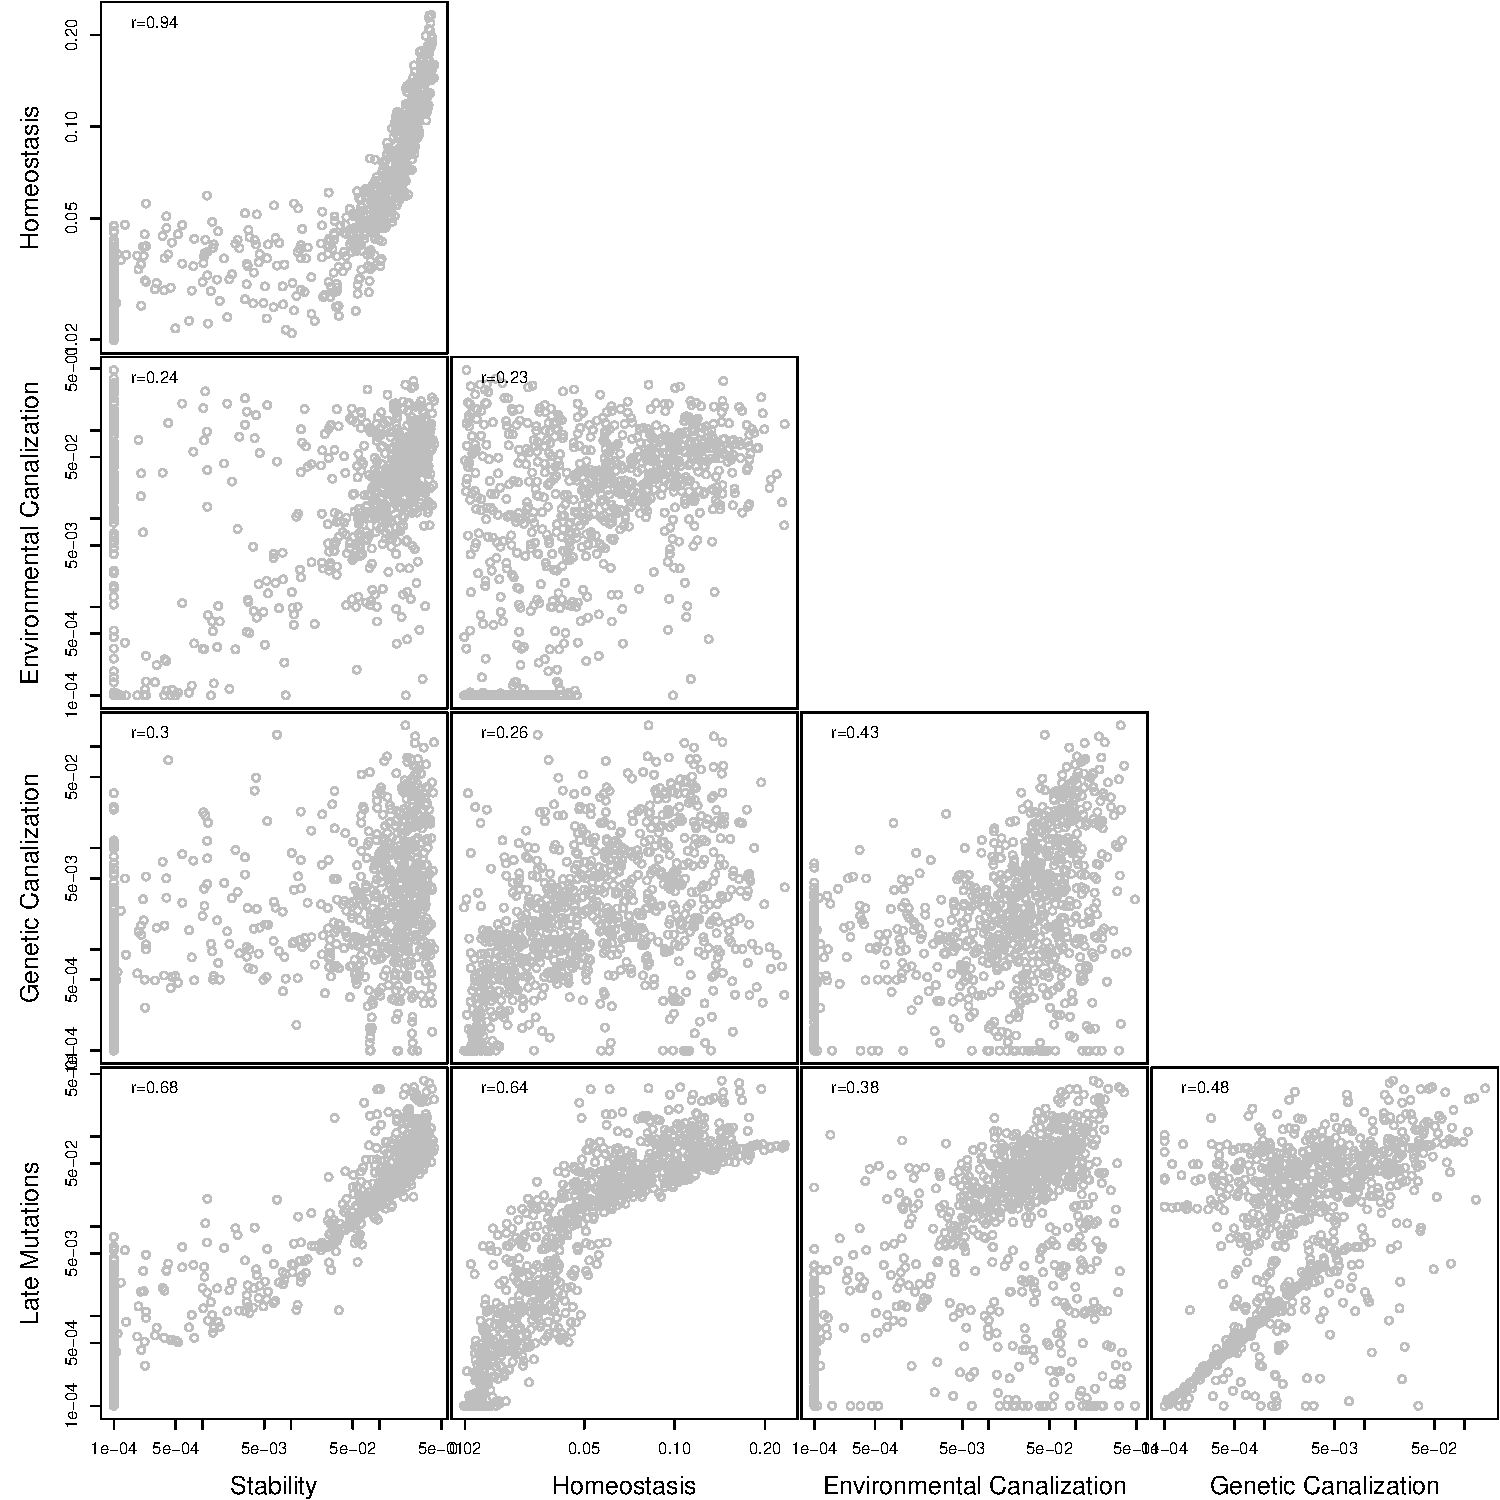
\includegraphics[width=15cm]{figures/R1-1-1b}
\caption{\label{fig:cor} Correlations between all five robustness components among 10,000 random 6-gene networks ($\mu_0=-0.2, \sigma_0=1.2$). Scatterplot axes are in log-scale ; correlation coefficients were calculated on the natural scale. }
\end{figure}

\clearpage
\begin{figure}[h!]
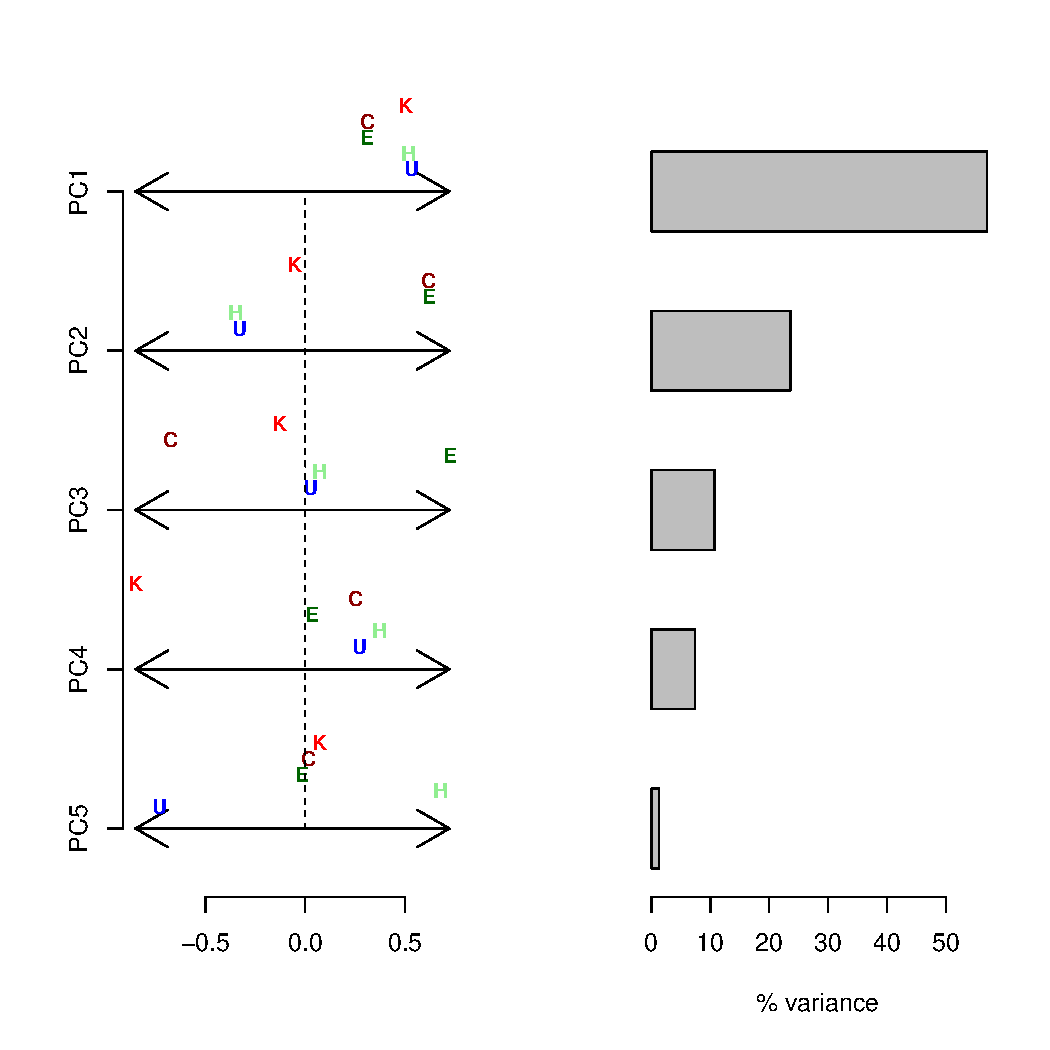
\includegraphics[width=10cm]{figures/R1-1-6}
\caption{\label{fig:pca} Summary of the principal component analysis on the five robustness components over 10,000 random 6-gene networks ($\mu_0=-0.2, \sigma_0=1.2$). Left: position of the five robustness components on all five Principal Components (PC). U: (un)stability, H: Homeostasis, E: Environmental canalization, C: Genetic canalization, K: Late mutation canalization. Right: relative contribution of the five PCs to the total variance.}
\end{figure}

\clearpage
\begin{figure}[h!]
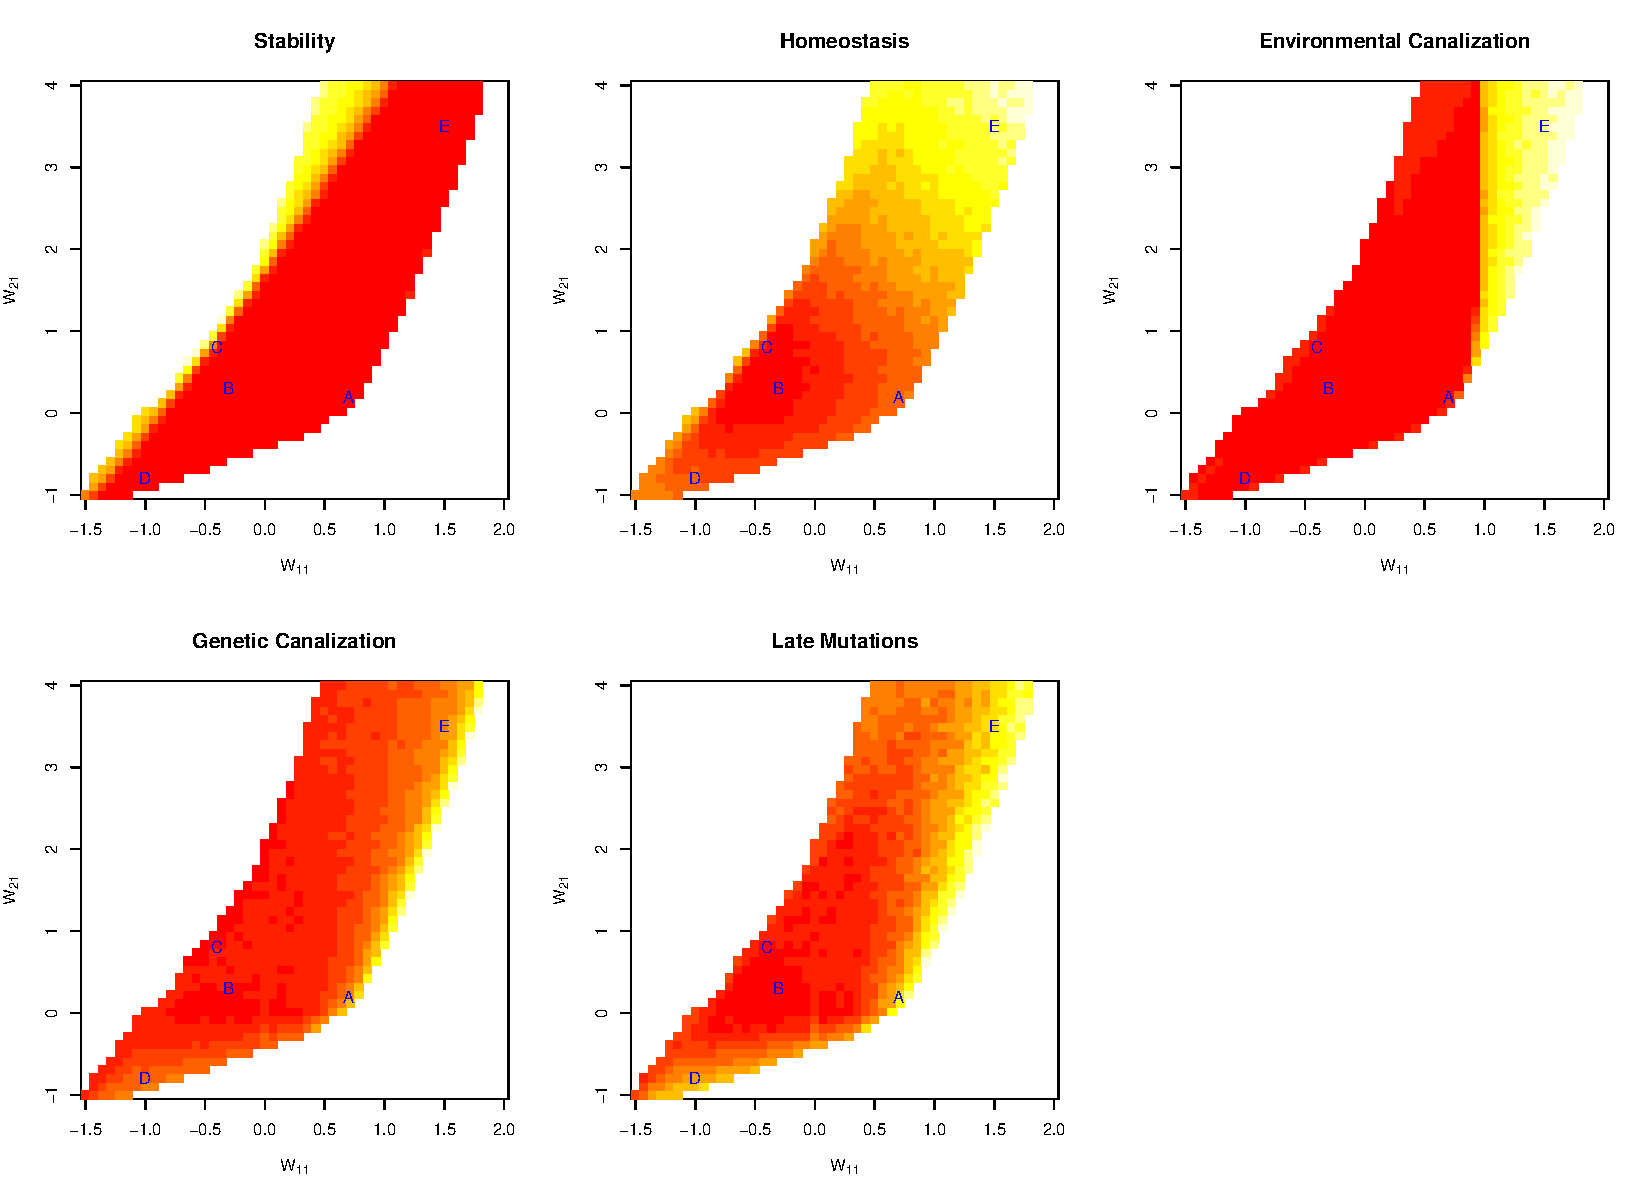
\includegraphics[width=15cm]{figures/T2-2-1}
\caption{\label{fig:imgpanels} Robustness indicators ($U$,$H$,$E$,$C$, and $K$, as described in the methods section) estimated for a continuum of two-gene networks with an equilibrium at $\bm S_\infty = (0.3, 0.6)$. Red stands for the maximum robustness (lowest scores); yellow for minimum robustness (highest scores). For readability, scales might be different between panels according of the range of the score (for instance, homeostasis ranges from 0.04 to 0.14 while stability ranges from 0 to 0.25). Letters A to E stand to five networks illustrated in figure~\ref{fig:simpanels}, and detailed in Table~\ref{tab:W}.}
\end{figure}

\clearpage
\begin{figure}[h!]
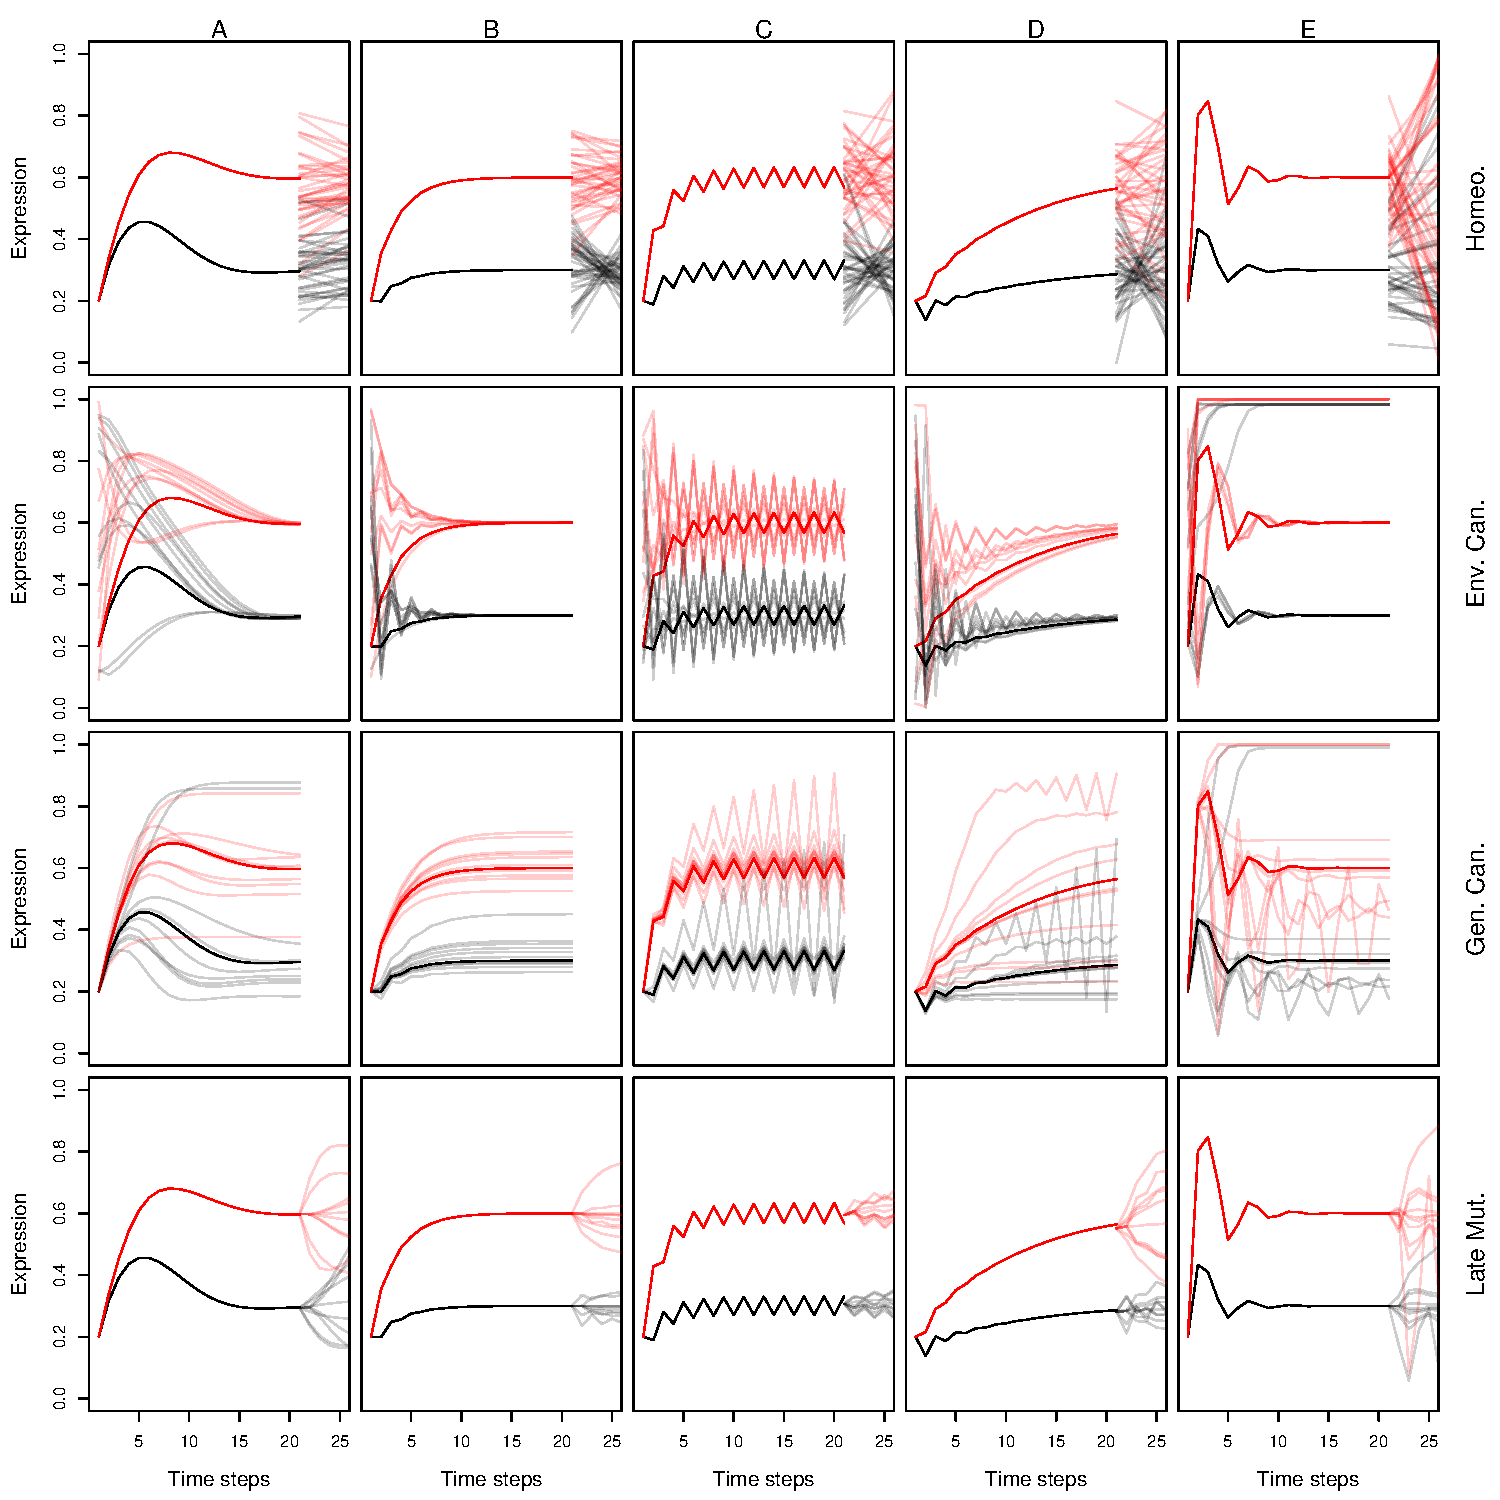
\includegraphics[width=15cm]{figures/T2-2-2}
\caption{\label{fig:simpanels} Illustration of the robustness scores for the five networks described in Table~\ref{tab:W}. In each panel, the default (undisturbed) network kinetics is displayed as plain lines (black for gene~1, red for gene~2). By construction, all networks have an equilibrium at (0.3, 0.6). The network stability can be assessed from the amplitude of the cycles in the undisturbed kinetics. Network homeostasis (first line) was estimated by disturbing the expression state of the genes (for readability, the network response was expanded over several time steps). Environmental canalization (second line) was estimated by disturbing the initial state (semi-transparent lines). Genetic canalization (third line) was measured as the variance in the final state when mutating the network at the beginning of the development. Finally, the robustness to late mutations (last line) consisted in mutating the network after having reached the equilibrium.  }
\end{figure}


\end{document}
